\documentclass{article}

\usepackage{amsmath,amssymb,amsthm,txfonts,gincltex}
\setlength{\oddsidemargin}{0.25 in}
\setlength{\evensidemargin}{-0.25 in}
\setlength{\topmargin}{-0.6 in}
\setlength{\textwidth}{6.5 in}
\setlength{\textheight}{8.5 in}
\setlength{\headsep}{0.75 in}
\setlength{\parindent}{0 in}
\setlength{\parskip}{0.1 in}

\newtheorem{theorem}{Theorem}
\newtheorem{corollary}{Corollary}
\newtheorem{proposition}{Proposition}
\newtheorem*{remark}{Remark}
\theoremstyle{definition}
\newtheorem{example}{Example}
\newtheorem{definition}{Definition}

\newcommand{\lecture}[4]{
   \pagestyle{myheadings}
   \thispagestyle{plain}
   \newpage
%   \setcounter{lecnum}{#1}
   \setcounter{page}{1}
   \noindent
   \begin{center}
   \framebox{
      \vbox{\vspace{2mm}
    \hbox to 6.58in { {\bf CSC~565: Graph Theory
                        \hfill North Carolina State University} }
    \hbox to 6.58in { {\bf Fall 2019
                        \hfill Computer Science} }
       \vspace{4mm}
       \hbox to 6.28in { {\Large \hfill Lecture #1: #2  \hfill} }
       \vspace{2mm}
       \hbox to 6.28in { {\it Lecturer: {\it Don Sheehy {\tt <drsheehy@ncsu.edu>}} \hfill Scribe: #4} }
      \vspace{2mm}}
   }
   \end{center}
   \markboth{Lecture #1: #2}{Lecture #1: #2}
   \vspace*{4mm}
}

\usepackage{graphics,tikz}
\usepackage{chngcntr}
\usepackage{caption}
\usepackage{capt-of}
\usepackage{sidecap}
\newtheorem{case}{Case}
\counterwithin*{case}{theorem}
\newtheorem{question}{Question}
\newtheorem{lemma}{Lemma}
\newtheorem{solution}[]{Solution}
%\def\geom{\text{geom}}
%\def\sim{\text{sim}}
%\def\R{\mathbb{R}}

\begin{document}

%FILL IN THE RIGHT INFO.
%\lecture{**LECTURE-NUMBER**}{**DATE**}{**LECTURER**}{**SCRIBE**}
\lecture{9}{Sep 23, 2019}{Don Sheehy}{Sharav Mathur, Kushal Batra, Nihal Narayanan }

\section{The Torus Graph(s)}
The \textit{Torus Graph} $T_{j,k}$ is a $j \times k$ grid with extra edges connecting the leftmost and rightmost vertex in each row as well as the top and bottom vertices of each column.

\begin{question}
    Prove that for any pair of vertices $a,b \in V_{T_{j,k}}$, there exists an isomorphism $f:T_{j,k} \to T_{j,k}$ such that $f(a) = b$.
\end{question}

\begin{proof}
    Consider a vertex $a \hspace{2pt} \epsilon \hspace{2pt} T_{j,k}$ in the form
    $(m,n)$ where $m \hspace{2pt} \epsilon \hspace{2pt} (0, 1, ... j-1)$ and $n \hspace{2pt} \epsilon \hspace{2pt} (0, 1, ... k-1)$. \\

    Its four adjacent vertices in the Torus graph would be
    \begin{align*}
        ((m+1)\%j, n) \\
        ((m-1)\%j, n) \\
        (m, (n+1)\%k) \\
        (m, (n-1)\%k) \\
    \end{align*}

    Consider any other vertex $b \hspace{2pt} \epsilon \hspace{2pt} T_{j,k}$ in the form $((m+x) \% j,(n+y) \% k)$. Changing $x$ and $y$, we get every other vertex in $T_{j,k}$.

    Consider the function $f$ that maps from $a$ to $b$ as 
    \begin{align*}
     f(a) = b
    \end{align*}

    then the following also holds true for its adjacent vertices:
    \begin{align*}
        f(((m+1)\%j, n)) = (((m+1)+x)\%j, n+y) = (((m+x)+1)\%j, n+y) \\
        f(((m-1)\%j, n)) = (((m-1)+x)\%j, n+y) = (((m+x)-1)\%j, n+y) \\
        f((m, (n+1)\%k)) = (m+x, ((n-1)+y)\%k) = (m+x, ((n+y)-1)\%k) \\
        f((m, (n+1)\%k)) = (m+x, ((n+1)+y)\%k) = (m+x, ((n+y)+1)\%k) \\
    \end{align*}

    From above, we can see that there is a bijective mapping, which when applied to $a$'s adjacent vertices, gives us $b$'s adjacent vertices. Since b is any vertex in the Torus graph, $T_{j,k}$, we can conclude that for any pair of vertices $a,b \in V_{T_{j,k}}$, there exists an isomorphism $f:T_{j,k} \to T_{j,k}$ such that $f(a) = b$.
\end{proof}

\begin{question}
    Prove that $T_{3,3}$ is $4$-connected
    \end{question}
\begin{proof}
    To prove that the graph is 4-connected, we need to show that $\forall u,v\hspace{2pt}\epsilon \hspace{2pt}$ $V_G$, $\exists$ four disjoint paths from $u$ to $v$.\\
    From the symmetry in the Isomorphism of the \textit{Torus Graph} shown in the above question, we are left with just\\
    two cases to prove that it is 4-connected.
    \begin{case}
        The two vertices are adjacent to each other. 
    \end{case}

\begin{center}
\begin{tikzpicture}[every node/.style={draw,circle,minimum size=7mm}]
\node[pink] (7) at (0,0) {7};
\node[pink] (8) at (2,0) {8};
\node[pink] (9) at (4,0) {9};
\node[pink] (4) at (0,2) {4};
\node (5) at (2,2) {5};
\node[pink] (6) at (4,2) {6};
\node (1) at (0,4) {1};
\node[pink] (2) at (2,4) {2};
\node[pink] (3) at (4,4) {3};
\draw[thick] (7) -- (8) -- (9) ;
\draw[thick] (4) -- (5) -- (6) ;
\draw[thick] (1) -- (2) -- (3) ;

\draw[thick] (7) -- (4) -- (1) ;
\draw[thick] (8) -- (5) -- (2) ;
\draw[thick] (9) -- (6) -- (3) ;


\draw[ultra thick, red] (1) -- (2) -- (5) ;
\draw[ultra thick, blue] (1) -- (4) -- (5) ;
\draw[ultra thick, blue] (1) -- (4) -- (5) ;
\draw[ultra thick, green] (7) -- (8) -- (5) ;
\draw[ultra thick, brown] (3) -- (6) -- (5) ;

\draw[ultra thick,green]   (1) to[out=80,in=-80] (7);
\draw   (2) to[out=80,in=-80] (8);
\draw   (3) to[out=80,in=-80] (9);
\draw[ultra thick,brown]   (1) to[out=170,in=10] (3);
\draw   (4) to[out=170,in=10] (6);
\draw   (7) to[out=170,in=10] (9);
\end{tikzpicture}
\end{center}

    \begin{case}
    The two vertices are diagonal to each other.
    \end{case}
\begin{center}
\begin{tikzpicture}[every node/.style={draw,circle,minimum size=7mm}]
\node[pink] (7) at (0,0) {7};
\node[pink] (8) at (2,0) {8};
\node[pink] (9) at (4,0) {9};
\node[pink] (4) at (0,2) {4};
\node[pink] (5) at (2,2) {5};
\node[pink] (6) at (4,2) {6};
\node (1) at (0,4) {1};
\node (2) at (2,4) {2};
\node[pink] (3) at (4,4) {3};
\draw[thick] (7) -- (8) -- (9) ;
\draw[thick] (4) -- (5) -- (6) ;
\draw[thick] (1) -- (2) -- (3) ;
\draw[thick] (7) -- (4) -- (1) ;
\draw[thick] (8) -- (5) -- (2) ;
\draw[thick] (9) -- (6) -- (3) ;


\draw[ultra thick, red] (1) -- (2);
\draw[ultra thick, blue] (1) -- (4) -- (5)--(2) ;
\draw[ultra thick, green] (7) -- (8);
\draw[ultra thick, brown] (3) -- (2) ;

\draw[ultra thick,green]   (1) to[out=80,in=-80] (7);
\draw[ultra thick,green]   (2) to[out=80,in=-80] (8);
\draw   (3) to[out=80,in=-80] (9);
\draw[ultra thick,brown]   (1) to[out=170,in=10] (3);
\draw   (4) to[out=170,in=10] (6);
\draw   (7) to[out=170,in=10] (9);
\end{tikzpicture}
\end{center}
    In \textbf{Case 1}, the four different colors show the four disjoint paths to reach from vertex 1 to vertex 5.\\
    In \textbf{Case 2}, the four different colors show the four disjoint paths to reach from vertex 1 to vertex 2.\\

    $\therefore \text{, From the above two diagrams it is easily observed that in both the cases, we are able to get four different paths that }$
    have no shared vertices (except the ends) from
    \text{source to destination.}\\
    \\This is another way of defining that the \textit{Torus Graph} $T_{3,3}$ is $4$-connected.
\end{proof}
\begin{question}
   Prove that if $j$ and $k$ are multiples of $3$, then there exists a Morphism from $T_{j,k}$ to $T_{3,3}$.
\end{question}
\begin{proof}
    Let $j = 3m$ and $k = 3n$.
    
    Consider the mapping $f$: \\
    \begin{gather*}
        f: T_{3m, 3n} \rightarrow T_{3,3} \\
        f_V((a, b)) = (a \% 3, b \% 3)
    \end{gather*}
    
    For the above mapping to be a Graph Morphism, we need to show that if there is an edge in $T_{3m,3n}$, then there is a corresponding edge in $T_{3,3}$
   
    For example, consider a vertical edge, $E = \{(a,b), ((a+1)\%3m, b) \hspace{2pt} \epsilon \hspace{2pt} T_{3m, 3n}$
    \begin{gather*}
    f_V((a+1)\%3m, b)) = (((a+1)\%3m)\% 3, b \% 3) \\
    \phantom{xxxxxxxxxx} = ((a+1)\% 3, b \% 3)
    \end{gather*}
    We know that $((a+1)\% 3, b \% 3) \hspace{2pt} \epsilon \hspace{2pt} T_{3, 3}$
    
    Similarly, we can also show this to be true for any horizontal edge. \\
    \begin{gather*}
     f_V((a, (b+1)\%3n)) = (a \% 3, ((b+1)\%3n)\% 3) \\
    \phantom{xxxxxxxxxxx} = (a \% 3, (b+1)\% 3) 
    \end{gather*}
    We know that $((a+1)\% 3, b \% 3) \hspace{2pt} \epsilon \hspace{2pt} T_{3, 3}$ and $(a \% 3, (b+1)\%3) \hspace{2pt} \epsilon \hspace{2pt} T_{3, 3}$
    
    $\implies \text{Hence, there exists a morphism from $T_{j,k}$ to $T_{3,3}$}$.
    
    \begin{center}
    
    \begin{tikzpicture}[every node/.style={draw,circle,minimum size=7mm}]
    
    \node (20) at (0,0) {20};
    \node (21) at (2,0) {21};
    \node (22) at (4,0) {22};
    \node (10) at (0,2) {10};
    \node (11) at (2,2) {11};
    \node (12) at (4,2) {12};
    \node (00) at (0,4) {00};
    \node (01) at (2,4) {01};
    \node (02) at (4,4) {02};
    \node (03) at (6,4) {03};
    \node (04) at (8,4) {04};
    \node (05) at (10,4) {05};
    \node (13) at (6,2) {13};
    \node (14) at (8,2) {14};
    \node (15) at (10,2){15};
    \node (23) at (6,0) {23};
    \node (24) at (8,0) {24};
    \node (25) at (10,0){25};
    
    \draw[thick] (20) -- (21) -- (22)--(23) -- (24) -- (25) ;
    \draw[thick] (10) -- (11) -- (12)-- (13) -- (14) -- (15) ;
    \draw[thick] (00) -- (01) -- (02) -- (03) -- (04) -- (05);
    \draw[thick] (20) -- (10) -- (00) ;
    \draw[thick] (21) -- (11) -- (01) ;
    \draw[thick] (22) -- (12) -- (02) ;
    \draw[thick] (23) -- (13) -- (03) ;
    \draw[thick] (24) -- (14) -- (04) ;
    \draw[thick] (25) -- (15) -- (05) ;
    
    
    \draw   (00) to[out=80,in=-80] (20);
    \draw   (03) to[out=80,in=-80] (23);
    \draw   (04) to[out=80,in=-80] (24);
    \draw   (05) to[out=80,in=-80] (25);
    \draw   (01) to[out=80,in=-80] (21);
    \draw   (02) to[out=80,in=-80] (22);
    \draw   (00) to[out=170,in=10] (05);
    \draw   (10) to[out=170,in=10] (15);
    \draw   (20) to[out=170,in=10] (25);
    \end{tikzpicture}
    \end{center}
\end{proof}


\begin{question}
    Prove that if $j\ge 3$ and $k\ge 3$, then $T_{j,k}$ contains a $T_{3,3}$ topological minor.  Recall that this means there is a subgraph of $T_{j,k}$ that can be transformed into $T_{3,3}$ by contracting paths of degree 2 vertices (i.e. induced paths) into a single edge.
\end{question}
\begin{proof}
    To prove the question, let us first take an example that satisfies the condition for $j\ge3$ and $k\ge3$.\\
    The Graph $T_{4,6}$ looks as shown below:
    
\begin{center}

\begin{tikzpicture}[every node/.style={draw,circle,minimum size=7mm}]
\node (30) at (0,-2) {30};
\node (31) at (2,-2) {31};
\node (32) at (4,-2) {32};
\node (33) at (6,-2) {33};
\node (34) at (8,-2) {34};
\node (35) at (10,-2) {35};

\node (20) at (0,0) {20};
\node (21) at (2,0) {21};
\node (22) at (4,0) {22};
\node (10) at (0,2) {10};
\node (11) at (2,2) {11};
\node (12) at (4,2) {12};
\node (00) at (0,4) {00};
\node (01) at (2,4) {01};
\node (02) at (4,4) {02};
\node (03) at (6,4) {03};
\node (04) at (8,4) {04};
\node (05) at (10,4) {05};
\node (13) at (6,2) {13};
\node (14) at (8,2) {14};
\node (15) at (10,2){15};
\node (23) at (6,0) {23};
\node (24) at (8,0) {24};
\node (25) at (10,0){25};

\draw[thick] (20) -- (21) -- (22)--(23) -- (24) -- (25) ;
\draw[thick] (10) -- (11) -- (12)-- (13) -- (14) -- (15) ;
\draw[thick] (00) -- (01) -- (02) -- (03) -- (04) -- (05);
\draw[thick] (30) -- (31) -- (32) -- (33) -- (34) -- (35);
\draw[thick]  (00) --(10) -- (20) -- (30) ;
\draw[thick] (01)--(11)--(21)--(31) ;
\draw[thick] (32)--(22) -- (12) -- (02) ;
\draw[thick] (33)--(23) -- (13) -- (03);
\draw[thick] (34)--(24) -- (14) -- (04);
\draw[thick] (35)--(25) -- (15) -- (05);

\draw   (00) to[out=80,in=-80] (30);
\draw   (03) to[out=80,in=-80] (33);
\draw   (04) to[out=80,in=-80] (34);
\draw   (05) to[out=80,in=-80] (35);
\draw   (01) to[out=80,in=-80] (31);
\draw   (02) to[out=80,in=-80] (32);
\draw   (00) to[out=170,in=10] (05);
\draw   (10) to[out=170,in=10] (15);
\draw   (20) to[out=170,in=10] (25);
\draw   (30) to[out=170,in=10] (35);
\end{tikzpicture}
\captionof{figure}{\textbf{Torus Graph $T_{4,6}$ }}
\end{center}
    For $T_{4,6}$ to contain a $T_{3,3}$ topological minor, we first have to take a subgraph of $T_{4,6}$. This is done to obtain vertices of degree 2.\\ \\
    For any general $T_{j,k}$, we apply the following three operations to obtain our subgraph: \\
    \begin{enumerate}
        \item For $x\ge0$ and $y\ge3$,  \\
        Remove edge between vertices (x,y) and (x+1\%j,y)
        \item For $x\ge3$ and $y\ge0$, \\
        Remove edges between vertices (x,y) and (x,y+1\%k)
        \item Remove all vertices (x,y) for $x\ge3$ and $y\ge3$.
    \end{enumerate}
    This subgraph, $H$ now looks as shown below:
\begin{center}

\begin{tikzpicture}[every node/.style={draw,circle,minimum size=7mm}]
\node (30) at (0,-2) {30};
\node (31) at (2,-2) {31};
\node (32) at (4,-2) {32};

\node (20) at (0,0) {20};
\node (21) at (2,0) {21};
\node (22) at (4,0) {22};
\node (10) at (0,2) {10};
\node (11) at (2,2) {11};
\node (12) at (4,2) {12};
\node (00) at (0,4) {00};
\node (01) at (2,4) {01};
\node (02) at (4,4) {02};
\node (03) at (6,4) {03};
\node (04) at (8,4) {04};
\node (05) at (10,4) {05};
\node (13) at (6,2) {13};
\node (14) at (8,2) {14};
\node (15) at (10,2){15};
\node (23) at (6,0) {23};
\node (24) at (8,0) {24};
\node (25) at (10,0){25};

\draw[thick] (20) -- (21) -- (22)--(23) -- (24) -- (25) ;
\draw[thick] (10) -- (11) -- (12)-- (13) -- (14) -- (15) ;
\draw[thick] (00) -- (01) -- (02) -- (03) -- (04) -- (05);
\draw[thick]  (00) --(10) -- (20) -- (30) ;
\draw[thick] (01)--(11)--(21)--(31) ;
\draw[thick] (32)--(22) -- (12) -- (02) ;

\draw   (00) to[out=80,in=-80] (30);
\draw   (01) to[out=80,in=-80] (31);
\draw   (02) to[out=80,in=-80] (32);
\draw   (00) to[out=170,in=10] (05);
\draw   (10) to[out=170,in=10] (15);
\draw   (20) to[out=170,in=10] (25);
\end{tikzpicture}
\end{center}
    Now from the subgraph, we obtain the desired minor by contracting paths of degree 2 vertices into a single edge.\\
    This is done by applying the following 2 operations:\\
    \begin{enumerate}
        \item Contract Path $P_1$ = $\{(x,2),(x,3)\dots(x,k-1),(x,0)\}$ to the Edge $\{(x,2),(x,0)\}$, for x $\epsilon$ $\{0,1,2\}$
        \item Contract Path $P_2$ = $\{(2,y),(3,y)\dots(j-1,y),(0,y)\}$ to the Edge $\{(2,y),(0,y)\}$, for y $\epsilon$ $\{0,1,2\}$
    \end{enumerate}
    
    Resulting graph is the Graph $T_{3,3}.$\\
    
    \begin{center}
\begin{tikzpicture}[every node/.style={draw,circle,minimum size=7mm}]
\node (20) at (0,0) {20};
\node (21) at (2,0) {21};
\node (22) at (4,0) {22};
\node (10) at (0,2) {10};
\node (11) at (2,2) {11};
\node (12) at (4,2) {12};
\node (00) at (0,4) {00};
\node (01) at (2,4) {01};
\node (02) at (4,4) {02};
\draw[thick] (20) -- (21) -- (22) ;
\draw[thick] (10) -- (11) -- (12) ;
\draw[thick] (00) -- (01) -- (02) ;

\draw[thick] (20) -- (10) -- (00) ;
\draw[thick] (21) -- (11) -- (01) ;
\draw[thick] (22) -- (12) -- (02) ;

\draw   (00) to[out=80,in=-80] (20);
\draw   (01) to[out=80,in=-80] (21);
\draw   (02) to[out=80,in=-80] (22);
\draw   (00) to[out=170,in=10] (02);
\draw   (10) to[out=170,in=10] (12);
\draw   (20) to[out=170,in=10] (22);
\end{tikzpicture}
\end{center}
    $\implies \text{Any Graph $T_{j,k}$ with $j\ge3$ and $k\ge3$ contains a $T_{3,3}$ minor }$
\end{proof}
\section{Graph Products}

\begin{question}
    Show that $K_2 \times K_2 \cong C_4$.
\end{question}

\begin{proof}
    In Graph theory, the Cartesian product 
    $G \times H$ of graphs $G$ and $H$ is a graph such that the vertex set
    of $G \times H$ is the Cartesian product $V(G) \times V(H)$; and two vertices $(u,u')$ and $(v,v')$ are adjacent in $G \times H$ if and only if either $u = v$ and $u'$ is adjacent to $v'$ in $H$, or $u' = v'$ and $u$ is adjacent to $v$ in $G$.
    
    Without any loss of generality, shown below are two $K_2$ graphs. \\
    
   \begin{center}

        \begin{tikzpicture}[every node/.style={draw,circle,minimum size=7mm}]
        
            \node (a) at (0,0) {a};
            
            \node (b) at (0,2) {b};
            
            \node (1) at (2,0) {1};
            
            \node (2) at (2,2) {2};
            
            \draw[thick] (1) -- (2) ;
            \draw[thick] (b) -- (a) ;
            \end{tikzpicture}
            \end{center}
            Below is their Cartesian Product.
            
            \begin{center}
            
            \begin{tikzpicture}[every node/.style={draw,circle,minimum size=7mm}]
            
            \node (a1) at (0,0) {a1};
            
            \node (b1) at (0,2) {b1};
            
            \node (a2) at (2,0) {a2};
            
            \node (b2) at (2,2) {b2};
            
            \draw[thick] (a1) -- (b1) -- (b2) -- (a2)--(a1) ;
            \draw[thick] (b) -- (a) ;
        \end{tikzpicture}
    \end{center}
    We can see that the resulting graph is a $C_4$.
\end{proof}

\begin{question}
    Show that $K_2 \times K_3$ can be drawn in the plane without crossing.
\end{question}

\begin{proof}
    Shown below are the two graphs $K_2$ and $K_3$ and their Cartesian product 
    $K_2 \times K_3$ \\ \\
    
    \begin{center}

\begin{tikzpicture}[every node/.style={draw,circle,minimum size=7mm}]

\node (a) at (0,0) {a};
\node (b) at (2,0) {b};
\node (c) at (1,2) {c};
\node (1) at (6,0) {1};
\node (2) at (6,2) {2};

\draw[thick] (a) -- (b) --(c)--(a) ;
\draw[thick] (1) -- (2) ;

\end{tikzpicture}
\end{center}
\vspace{8pt}  
\begin{center}

\begin{tikzpicture}[every node/.style={draw,circle,minimum size=7mm}]

\node (a1) at (0,0) {a1};

\node (b1) at (2,0) {b1};

\node (c1) at (1,2) {c1};
 
\node (a2) at (-2,-2) {a2};

\node (b2) at (4,-2) {b2};

\node (c2) at (1,4) {c2};
 
 

\draw[thick] (a1) -- (b1) --(c1)--(a1) ;
\draw[thick] (a2) -- (b2) --(c2)--(a2) ;
\draw[thick] (a1) -- (a2) ;
\draw[thick] (b1) -- (b2) ;
\draw[thick] (c1) -- (c2) ;
\end{tikzpicture}
\end{center}\
    
    
    The resulting graph can be drawn in the plane without crossing. \\
    We can also see that this Graph does not contain any $K_{3,3}$ or $K_5$ minors or equivalently no $K_{3,3}$ or $K_5$ topological minors. From \textbf{Kurtowski's Theorem}, we have that the Graph is planar.
\end{proof}


\begin{question}
    Prove that if $B$ is connected, then $A$ is a minor of $A\times B$ by giving a surjective simplicial map with connected preimages. 
\end{question}

\begin{proof}
    Let us check the following mapping $f$ from $A \times B$ to $A$
  \begin{gather*}
      f: A \times B \rightarrow A \\
      f_V: (a, b) \rightarrow a \\
      f_E: \{ (a,b), (a,b') \} \rightarrow \{a, a\} = \{a\} \\
      f_E: \{ (a,b), (a',b) \} \rightarrow \{a, a'\} \hspace{2pt}  \epsilon \hspace{2pt} E_A
    \end{gather*}
    
    To show that $A$ is a minor of $A \times B$, we need to show that firstly, the mapping above is surjective and secondly, that the pre-images are connected.
    \begin{enumerate}
        \item The mapping is surjective because under the mapping $f_V$, there are $|V_B|$ pre-images for every vertex $a \hspace{2pt} \epsilon  \hspace{2pt}A$.
        \item If we take the pre-image of any vertex $a \hspace{2pt} \epsilon \hspace{2pt} A$, then we get the set
    $\{ (a,b) \hspace{2pt}|\hspace{2pt} b \hspace{2pt} \epsilon \hspace{2pt} V_B \}$. From the definition of the Cartesian product and the fact that $B$ is connected, we can conclude that the pre-image is also connected.
    \end{enumerate}
    
\end{proof}


\begin{question}
    Show that $C_j \times C_k \cong T_{j,k}$
\end{question}

\begin{proof}
Consider the cycles
\begin{align*}
C_j = (\{0, 1, .. j-1 \}, \{(m, {(m+1)\%j})\hspace{2pt} | \hspace{2pt} m \hspace{2pt} \epsilon \hspace{2pt} \{ 0, 1, ... j-1 \} \}) \\
C_k = (\{ 0, 1, ... k-1 \}, \{(n, {(n+1)\%k})\hspace{2pt} | \hspace{2pt} n \hspace{2pt} \epsilon \hspace{2pt} \{ 0, 1, ... k-1 \} \})
\end{align*}
In $C_j \times C_k$, we have from the definition of Cartesian product that,
\begin{align*}
\{(m,n), ((m+1)\%j, n)\} \hspace{2pt} \epsilon \hspace{2pt} E_{C_j \times C_k}\\
\{(m,n), (m, (n+1)\%k)\} \hspace{2pt} \epsilon \hspace{2pt} E_{C_j \times C_k}
\end{align*}
\begin{center}
where $m \hspace{2pt} \epsilon \hspace{2pt} \{ 0, 1, ... j-1 \}$ and  $n \epsilon \{ 0, 1, ... k-1 \}$
\end{center}
For example, consider Graphs $C_3$ and $C_4$. Their Cartesian product is shown below\\

\begin{center}

\begin{tikzpicture}[every node/.style={draw,circle,minimum size=7mm}]

\node (1) at (0,0) {1};
\node (2) at (0,2) {2};
\node (3) at (0,4) {3};

\draw[thick] (1) -- (2) -- (3) ;


\draw   (3) to[out=80,in=-80] (1);
\end{tikzpicture}
\end{center}
\begin{center}


\begin{tikzpicture}[every node/.style={draw,circle,minimum size=7mm}]

\node (a) at (0,4) {a};
\node (b) at (2,4) {b};
\node (c) at (4,4) {c};
\node (d) at (6,4) {d};

\draw[thick] (a) -- (b) -- (c) -- (d);


\draw   (a) to[out=170,in=10] (d);
\end{tikzpicture}
\end{center}



\begin{center}

\begin{tikzpicture}[every node/.style={draw,circle,minimum size=7mm}]

\node (a1) at (0,0) {a1};
\node (b1) at (2,0) {b1};
\node (c1) at (4,0) {c1};
\node (d1) at (6,0) {d1};
\node (a2) at (0,2) {a2};
\node (b2) at (2,2) {b2};
\node (c2) at (4,2) {c2};
\node (d2) at (6,2) {d2};
\node (a3) at (0,4) {a3};
\node (b3) at (2,4) {b3};
\node (c3) at (4,4) {c3};
\node (d3) at (6,4) {d3};

\draw[thick] (a1) -- (b1) -- (c1) -- (d1);
\draw[thick] (a2) -- (b2) -- (c2) -- (d2);
\draw[thick] (a3) -- (b3) -- (c3) -- (d3);
\draw[thick] (a1) -- (a2) -- (a3) ;
\draw[thick] (b1) -- (b2) -- (b3) ;
\draw[thick] (c1) -- (c2) -- (c3) ;
\draw[thick] (d1) -- (d2) -- (d3) ;


\draw   (d1) to[out=-80,in=80] (d3);
\draw   (a3) to[out=80,in=-80] (a1);
\draw   (b3) to[out=80,in=-80] (b1);
\draw   (c3) to[out=80,in=-80] (c1);
\draw   (a3) to[out=170,in=10] (d3);
\draw   (a3) to[out=170,in=10] (d3);
\draw   (a2) to[out=170,in=10] (d2);
\draw   (a1) to[out=170,in=10] (d1);
\end{tikzpicture}
\end{center}

$\therefore$ Every vertex in $C_j \times C_k$ is connected to its four neighbours in a cyclic fashion which is nothing but the Torus graph $T_{j,k}$
\end{proof}



\section{Euler Walks}
For all of the questions below, let $G$ be a graph with exactly four vertices $a,b,c,d$ of odd degree.
Let $W$ be the edges of a walk from $a$ to $b$ that does not repeat any edges.\\

\begin{question}
    Prove that $c$ and $d$ are connected even if we remove the edges of $W$.  That is, $c$ and $d$ are connected in $G' = G\setminus W\setminus \{v \hspace{4pt} \epsilon \hspace{4pt} (G\setminus W)\hspace{2pt} |\hspace{2pt} deg(v) = 0\}$.

\end{question}
\begin{proof}
    The walk $W$ from $a$ to $b$ does not repeat any edges. In Graph $G'$, we remove the edges from G, which are part of the Walk and any isolated vertices that are left after removing it.\\
    \\
    Also, for any vertex other than $a$ and $b$, when you enter the vertex you also have to leave it.\\
    $\implies \text{In $G'$, parity of all the degree of vertices remains the same, except the source and destination vertices.}$\\
    \\ To summarise :
    \begin{enumerate}
        \item Parity of degree of vertices $a$ and $b$ changes from odd to even.\\
        \item Parity of degree of vertices of $c$ and $d$ remains odd.\\
        \item Parity of degree for all other vertices remains even.
    \end{enumerate}
    The Graph $G'$ may now have one or more connected components.\\
    Let us consider two cases depending upon where $c$ and $d$ are located.\\
    \begin{case}
        If $c$ and $d$ are part of different (connected)components.\\
        \\
        Let us assume that $c$ and $d$ are in fact not in the same connected component. We prove by contradiction using \textit{Handshake Lemma} that this case is not possible. 
        
        \begin{lemma}  \textit{Handshake Lemma}\\
            Number of vertices of odd degree in a graph is even
        \end{lemma}
        
        If one connected component has vertex $c$ but not $d$, this would mean that $c$ is the only vertex of that connected component with odd degree, while all other vertices are of even degree.\\
        \textit{Handshake Lemma} clearly states that this is not possible.\\
        \\
    \end{case}
    \begin{case}
        If $c$ and $d$ are part of the same (connected)component.\\
        \\
        In this case, $c$ and $d$ are the only odd degree vertices of the component, while all other vertices have even degree.\\
        By \textbf{Euler's Theorem}, $\exists \text{ an Euler Walk from $c$ to $d$.}$
        \\
        $\implies \text{$c$ and $d$ are connected.}$
    \end{case}
    

    $\therefore \text{Only Case 2 is possible.\\ Vertices $c$ and $d$ are connected.}$
\end{proof}

\begin{question}
    Suppose that $W$ is the longest such walk and that $G$ is connected.  Prove that in this case, $G'$ is connected.
\end{question}
\begin{proof}
    Let us take Graph G as the following\\
\begin{center}

\begin{tikzpicture}[every node/.style={draw,circle,minimum size=7mm}]

\node (v) at (0,0) {v};

\node (d) at (1,2) {d};

\node (b) at (1,4) {b};

\node (u) at (0,6) {u};

\node (c) at (-1,2) {c};

\node (a) at (-1,4) {a};

\draw[thick] (u) -- (a) ;
\draw[thick] (c) -- (a) ;
\draw[thick] (b) -- (d) ;
\draw[thick] (c) -- (v);
\draw[thick] (v) -- (d) ;
\draw[thick] (b) -- (u);
\draw[thick] (b) -- (a);

\draw[thick] (c) -- (d);

\end{tikzpicture}
\end{center}
    The longest walk, $W$ from $a$ to $b$ can be denoted by the sequence of vertices ($a$,$b$,$u$,$a$,$c$,$v$,$d$,$b$).\\
    \\
    $G' = G\setminus W\setminus \{v \hspace{4pt} \epsilon \hspace{4pt} (G\setminus W)\hspace{2pt} |\hspace{2pt} deg(v) = 0\}$\\
    \\
    $\implies \text{G' = \{\{c,d\},(c,d)\}}$
\begin{center}

\begin{tikzpicture}[every node/.style={draw,circle,minimum size=7mm}]

\node (d) at (1,2) {d};
\node (c) at (-1,2) {c};

\draw[thick] (c) -- (d);

\end{tikzpicture}
\end{center}

    Every time, we do this operation of removing the longest walk, we will get only one connected component.\\
    This is true because let us suppose after removing walk $W$ from $G$, we got more than 1 connected component.

\begin{enumerate}
    \item First component would have both vertices $c$ and $d$ together. This was shown in the previous question using the \textit{Handshake Lemma}.
    \item Second, or any other, component would have all vertices with even degree.\\
    By \textbf{Euler's Theorem}, we know that a connected Graph with all even degree vertices has an \textit{Euler Tour.}\\
    This is contradiction to the fact that we've chosen the longest walk.
    \end{enumerate}
    
    \text{[NOTE : We could've added the Euler Tour to the existing walk and gotten an even longer walk.]}

    $\implies \text{There is only one connected component in $G'$ and therefore, $G'$ is a connected Graph.}$\\
    \\
\end{proof}

\begin{question}
    Prove that if $G$ is connected, then there is a pair of walk that don’t repeat any edges, don’t have any edges in common, and together, touch every edge of $G$.
\end{question}
\begin{proof}
    It follows from the previous question that if $G$ is connected if we take the longest walk W from $a$ to $b$, then Graph $G'$ is still connected.
    \\ \\
    Again, by \textbf{Euler Theorem}, a connected graph with all even degree vertices except two vertices (source and destination) as odd degree vertices, has an \textit{Euler Walk} from the source to destination. Let this be denoted by W2.
    \\ \\
    $\implies \text{In Graph $G'$, as only $c$ and $d$ vertices have odd degree, while all other vertices have even degree, there exists an}$ \\ \textit{Euler} \text{from $c$ to $d$.}
    
    $\therefore \text{Walks W and W2 don't repeat any edges, don't have any edges in common, and together, touch every edge of Graph $G$.}$
\end{proof}
\end{document}